\documentclass[tikz, preview]{standalone}

\usepackage{amsfonts, amsthm, amssymb, amsmath, stmaryrd, etoolbox}
\usepackage{tikz}
\usetikzlibrary{matrix,arrows}

\begin{document}
\[
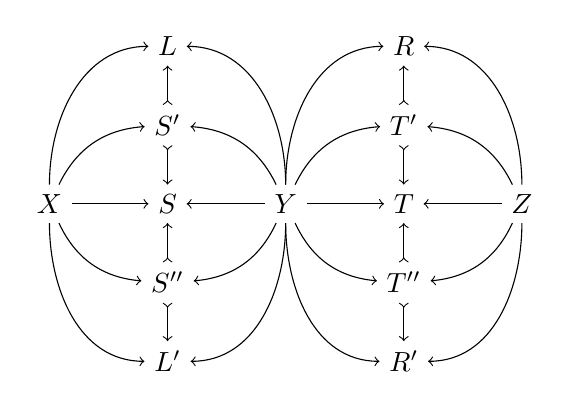
\begin{tikzpicture}
\node (X) at (-4,0) {$X$};
\node (Y) at (-1,0) {$Y$};
\node (Z) at (2,0) {$Z$};
\node (L) at (-2.5,2) {$L$};
\node (S') at (-2.5,1) {$S'$};
\node (S) at (-2.5,0) {$S$};
\node (S'') at (-2.5,-1) {$S''$};
\node (L') at (-2.5,-2) {$L'$};
\node (R) at (0.5,2) {$R$};
\node (T') at (0.5,1) {$T'$};
\node (T) at (0.5,0) {$T$};
\node (T'') at (0.5,-1) {$T''$};
\node (R') at (0.5,-2) {$R'$};
%
\draw [->] (X) edge[out=90,in=180] (L);
\draw [->] (X) edge[bend left=30] (S');
\draw [->] (X) edge (S);
\draw [->] (X) edge[bend right=30] (S'');
\draw [->] (X) edge[out=-90,in=180] (L');
\draw [->] (Y) edge[out=90,in=0] (L);
\draw [->] (Y) edge[bend right=30] (S');
\draw [->] (Y) edge (S);
\draw [->] (Y) edge[bend left=30] (S'');
\draw [->] (Y) edge[out=-90,in=0] (L');
\draw [->] (Y) edge[out=90,in=180] (R);
\draw [->] (Y) edge[bend left=30] (T');
\draw [->] (Y) edge (T);
\draw [->] (Y) edge[bend right=30] (T'');
\draw [->] (Y) edge[out=-90,in=180] (R');
\draw [->] (Z) edge[out=90,in=0] (R);
\draw [->] (Z) edge[bend right=30] (T');
\draw [->] (Z) edge (T);
\draw [->] (Z) edge[bend left=30] (T'');
\draw [->] (Z) edge[out=-90,in=0] (R');
\draw [>->] (S') edge (L);
\draw [>->] (S') edge (S);
\draw [>->] (S'') edge (S);
\draw [>->] (S'') edge (L');
\draw [>->] (T') edge (R);
\draw [>->] (T') edge (T);
\draw [>->] (T'') edge (T);
\draw [>->] (T'') edge (R');
%
\end{tikzpicture}
\]
\end{document}
